Основополагающим подходом в проектировании модуля конфигурируемой перестановки \texttt{remap} является создание таких элементарных устройств, которые способны принимать на вход весь требуемый объём данных и формировать из него лишь один выходной канал. Это обеспечивает высокую гибкость в масштабировании, поскольку в таком случае реализация необходимого количества выходных каналов достигается простой репликацией подобных структур, как это показано на рисунке \ref{fig:remap_replication}.\par

\begin{figure}[ht]
    \centering
    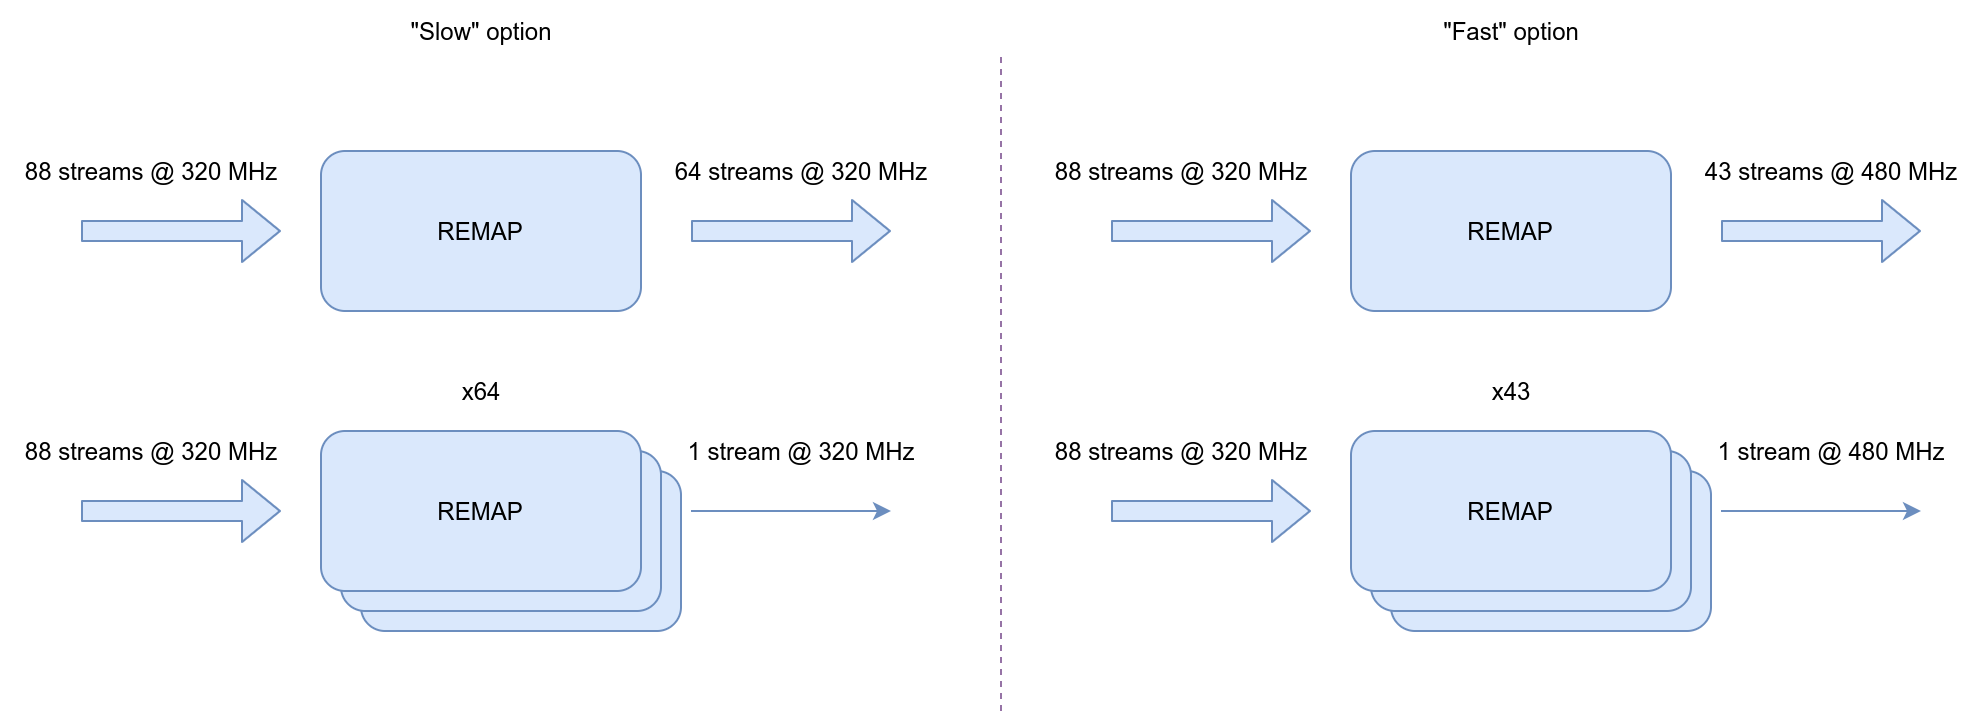
\includegraphics[width=\linewidth]{remap_replication.png}
    \caption{Схема формирования необходимого количества выходных каналов}
    \label{fig:remap_replication}
\end{figure}\par

Стоит отметить, поскольку входной поток данных разбивается на 4 независимые части, обрабатывающиеся отдельно, каждый модуль \texttt{remap} должен принимать лишь 22 канала и формировать 16 или 11 выходов, в зависимости от варианта сигнального процессора LASP.\par
В ходе разработки было спроектировано и реализовано два различных варианта архитектуры базового элемента модуля \texttt{remap}: с модулем синхронизации тактовых доменов, а также архитектура, основанная на FIFO памяти.\par
Во всех вариантах архитектуры можно выделить три основных этапа обработки:\par
\begin{itemize}
    \item предварительная перестановка данных в рамках каждого входного канала;
    \item извлечение из потока интересующих значений и их запись в память;
    \item чтение сохранённых данных из памяти в корректном порядке.
\end{itemize}\par
Первый этап обработки реализуется с помощью внешнего модуля Ialign и заключается в переупорядочивании значений АЦП в пределах каждого отдельного канала данных. Для корректной работы модуля \texttt{remap} требуется подобрать такую конфигурацию этих перестановок по всем каналам, чтобы значения, предназначенные для любого выходного канала не пересекались по временным ячейкам.\par
На втором этапе данные поступают на мультиплексор, который захватывает лишь один канал на каждом из тактов. Именно для этой операции и требуется условие первого этапа -- если одномоментно несколько входных каналов будут содержать значения, предназначенные для одного выходного, то часть данных будет просто пропущена. Это ограничение особенно важно для варианта сигнального процессора LASP с медленной опцией: как на входных интерфейсах, так и на выходных для каждого столкновения пучков передаётся по 8 величин, поэтому крайне необходимо, чтобы на каждом такте было доступно нужное значение. В быстрой опции выходной интерфейс имеет по 12 ячеек с данными, что вынуждает размещать два мультиплексора, ведь одного не будет достаточно в любом случае. В таком раскладе допускается одновременное наличие не более двух активных каналов для каждого базового блока модуля конфигурируемой перестановки. Извлечённые из общего потока значения, предназначенные для определённого выходного канала, временно буферизируются в памяти.\par
После накопления всех необходимых значений АЦП их необходимо переупорядочить, что осуществляется просто путём считывания данных в требуемой последовательности, согласно конфигурации. Стоит отметить, что буферизация данных в памяти позволяет обеспечить их безопасный переход из тактового домена $f_{feb}$ в домен $f_{core}$.\par

\subsubsection{Архитектура с модулем синхронизации тактовых доменов}
Первый вариант архитектуры компонента Remap, содержащий специальный модуль синхронизации тактовых доменов, представлен на рисунке \ref{fig:remap_cds}.\par
\begin{figure}[ht]
    \centering
    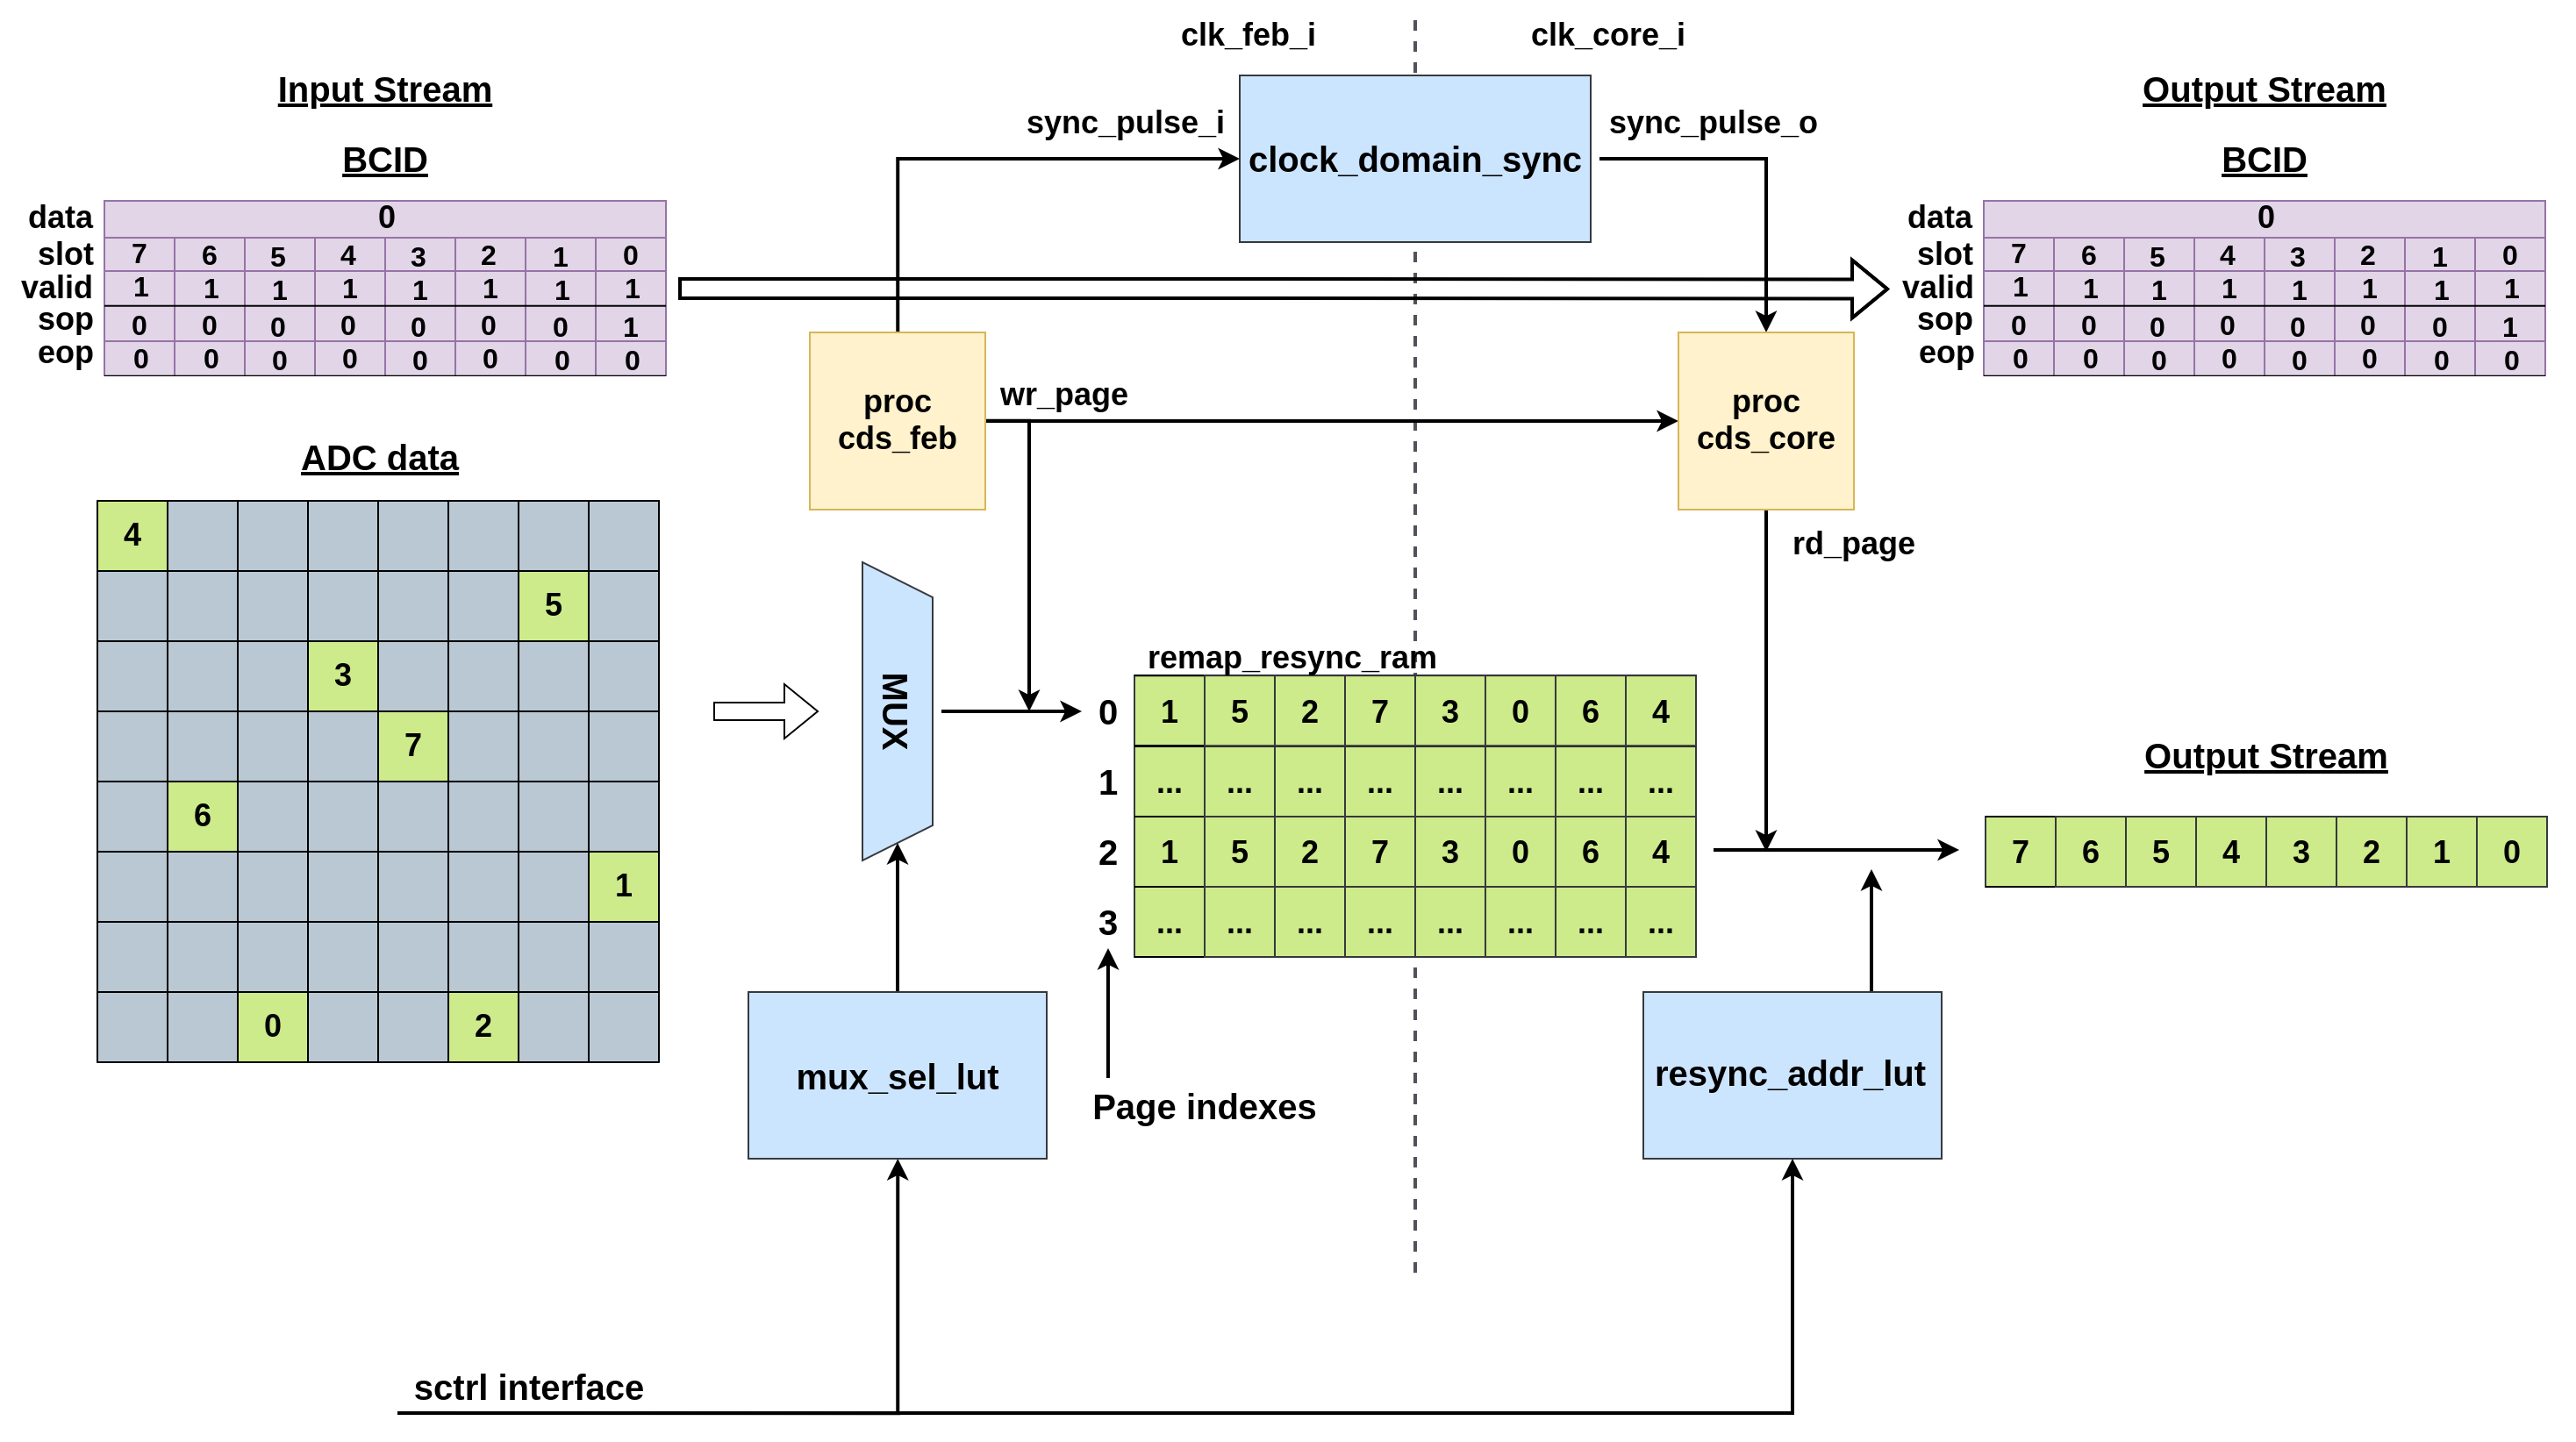
\includegraphics[width=\linewidth]{remap_cds.png}
    \caption{Схема архитектуры модуля Remap с модулем синхронизации тактовых доменов ПЕРЕВЕСТИ}
    \label{fig:remap_cds}
\end{figure}\par
Основной особенностью этой архитектуры является то, что в качестве буфера для мультиплексированных данных используется блок двухпортовой RAM памяти. Эта память разбита на несколько страниц, каждая из которых имеет размер, достаточный для хранения захваченной информации, относящейся к одному столкновению пучков. Чтение данных из страницы начинается лишь только после её полного заполнения записывающей стороной. Для синхронизации процессов считывания и записи предусмотрен следующий механизм: по завершению заполнения страницы памяти записывающая логика генерирует импульс шириной в один такт и отправляет его на вход специального модуля. Внутри этого модуля расположены два счётчика, работающие на тактовых частотах $f_{feb}$ и $f_{core}$, которые ведут счёт в диапазоне количества временных ячеек для каждого BCID. В рабочем режиме первый настроен так, чтобы обнуляться одновременно с поступлением синхросигнала от записывающей логики, а второй с задержкой около такта $f_{feb}$ после первого. При завершении цикла работы второго счётчика формируется выходной сигнал синхронизации, который поступает к считывающей логике и означает, что очередная страница в двухпортовой памяти заполнена полностью и можно безопасно извлекать из неё данные. Если вдруг синхронизация собьётся и синхросигнал от системы записи придёт не вовремя, то модуль это обнаружит и перейдёт в режим восстановления синхронизации. Часть данных после сбоя синхронизации будет утеряно, но через некоторое время система автоматически восстановится и продолжит работать исправно.\par
Описанная архитектура была реализована на языке описания цифровой логики VHDL и отлажена. По результатам тестирования в симуляторе она подтвердила свою работоспособность. Однако такой подход имеет ряд недостатков, главным из которых является необходимость передавать целый набор сигналов(такие как номер текущей страницы, индекс столкновения пучка, а также ряд вспомогательных сигналов внутри модуля синхронизации тактовых доменов) между тактовыми доменами $f_{feb}$ и $f_{core}$ вручную, используя схемы на двух регистрах. Для корректной организации таких переходов требуется тонкая ручная настройка временных ограничений, реализуемая путём составления специальных указаний синтезатору физической схемы, входящему в состав программного комплекса Intel Quartus Prime. Это значительно усложняет весь проект и делает его гораздо менее гибким. После возникновения проблем с разводимостью логики проекта LATOME, который является основой задетекторной электроники эксперимента ATLAS, разработанной в рамках предшествующей фазы обновления детектора, командой разработчиков сигнального процессора LASP было принято решение максимально избегать подобные способы перехода между тактовыми доменами. Кроме того, данный вариант является довольно путанным и сложным для понимания в деталях. Учитывая все эти недостатки, было решено разработать альтернативную архитектуру модуля Remap.\par


\subsubsection{Архитектура, основанная на FIFO}
Второй вариант архитектуры компонента Remap, содержащий память FIFO, представлен на рисунке \ref{fig:remap_fifo}.\par
\begin{figure}[ht]
    \centering
    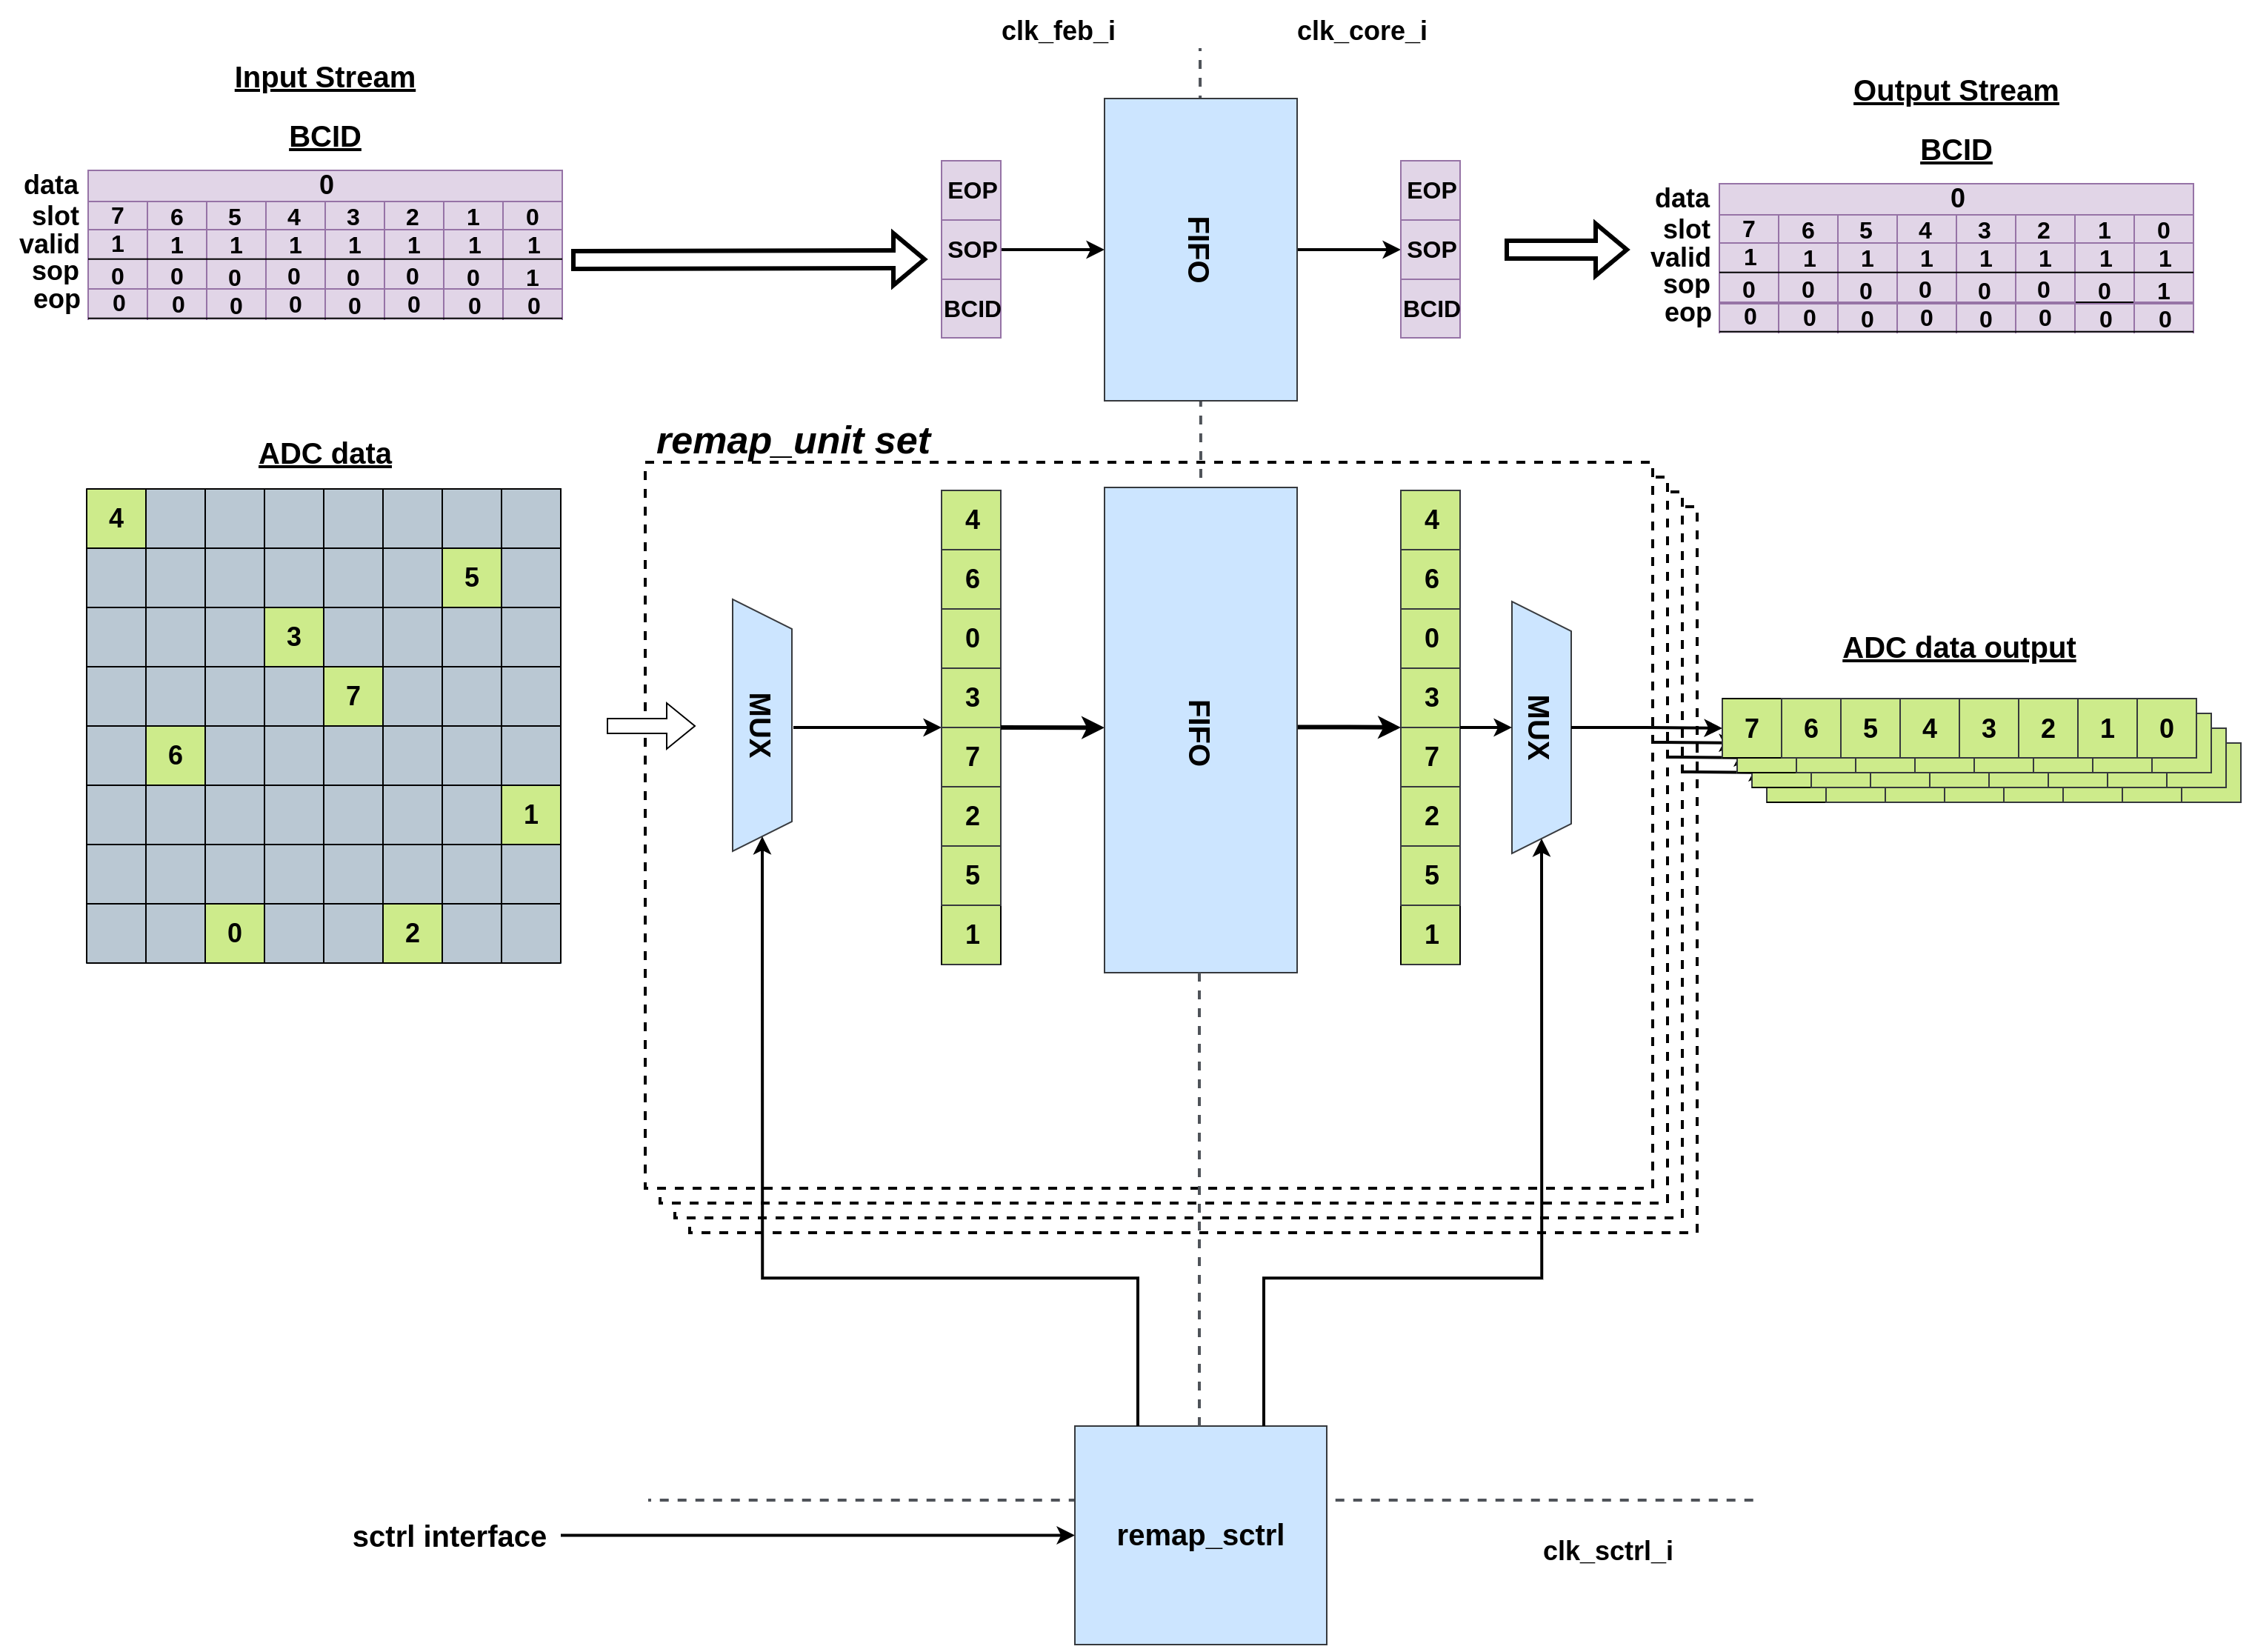
\includegraphics[width=\linewidth]{remap_fifo.png}
    \caption{Схема архитектуры модуля Remap, основанной на FIFO ПЕРЕВЕСТИ}
    \label{fig:remap_fifo}
\end{figure}\par
В рамках данного подхода в качестве буфера для мультиплексированных данных является память FIFO (First In First Out). Такая структура состоит из двухпортовой памяти, двух счётчиков адреса и двух автоматов для чтения и записи данных и является одним из ключевых элементов цифровой схемотехники. Одно из самых распространённых применений такой памяти, помимо буферизации информации -- это реализация перехода данных между тактовыми доменами. Поскольку такая память используется невероятно часто в проектировании логических схем, то существует множество готовых вариантов их реализации, в том числе и от разработчиков самих микросхем ПЛИС и соответствующего программного обеспечения для автоматического проектирования, в том числе и от Intel. В случае использования такого готового блока FIFO не требуется ручное написание временных ограничений, что избавляет от потенциальных проблем на этапе синтеза цифровой схемы всего проекта.\par
Однако, одна из основных особенностей FIFO -- это сохранение порядка записываемых данных, что не позволяет реализовать последний этап работы модуля Remap. Для решения данной задачи используется подход, при котором данные с мультиплексора поступают не напрямую на вход FIFO, а записываются в один большой регистр, достаточного размера для одновременного хранения всех мультиплексированных данных в рамках текущего столкновения пучков. Для наиболее оптимального использования логических ресурсов этот регистр является сдвиговым, то есть каждый такт новое значение поступает в начало, после чего оно смещается дальше. Только после полного заполнения этого регистра актуальными величинами, данные одним большим словом записывается в FIFO. Считывающая логика, после обнаружения данных на выходе FIFO, имеет доступ сразу ко всем значениям и может извлекать их последовательно в необходимом порядке.\par
В целях минимизации латентности необходимо, чтобы поступающие в FIFO данные сразу же были доступны для чтения, то есть требуется не допускать его заполнения. Поскольку запись и извлечение идёт с одной и той же скоростью, важно важно сделать так, чтобы считывающая система начала работу как минимум не позднее записывающей. Это достигается правильным управлением сигналами сброса: после старта сигнального процессора LASP сначала должен сняться сброс, синхронный с тактовым доменом $f_{core}$, а уже затем $f_{feb}$.\par

